\documentclass[12pt, a4paper]{article}
\usepackage{CJKutf8}
\usepackage[left=2cm, right=2cm, top=3cm, bottom=2.5cm]{geometry}
\usepackage[nodayofweek,level]{datetime}
\usepackage{comment}

%..This section controls the header-footer layout of the document
\usepackage{fancyhdr}
\pagestyle{fancy}
\lhead{Machine Learning (NTU CSIE, Fall 2017)}
\chead{}
\rhead{Instructor: Hsuan-Tien Lin}
\renewcommand{\headrulewidth}{0.4pt}

%..This section controls the title layout
\title{\vspace{-4ex}\bf{\LARGE{Homework \#3}}} 
\author{資工三\space\space\space B04902009\space\space\space 蕭千惠} % \footnote{blablabla} 
\date{\vspace{-2ex}\today\vspace{-4ex}}
%{\formatdate{21}{2}{2017}}

%.. math
\usepackage{mathtools}
\usepackage{amssymb}
\usepackage{amsmath}
\usepackage{upgreek}
\usepackage{bm}

%.. hyperlink / url
\usepackage[hyphens]{url}
\usepackage{hyperref}
\hypersetup{
    colorlinks=true,
    linkcolor=blue,
    filecolor=magenta,      
    urlcolor=blue,
}
\urlstyle{same}
%%\url{url}
%%\herf{url}{words to show}

% .. Include graph
\usepackage{graphicx}
% \includegraphics[width=16.5cm, keepaspectratio=true]{wireless_CSIE_server.png} \par

%.. change font size
\usepackage{type1cm}

%.. change enumerate label
\usepackage{enumitem}
%%\begin{enumerate}[label=(\alph*)]  //(a) (b) (c)
%%\begin{enumerate}[label=(\Alph*)]  //(A) (B) (C)
%%\begin{enumerate}[label=(\roman*)] //(i) (ii) (iii`')
\usepackage{amsfonts}
\usepackage{stmaryrd}
\usepackage{physics}	%partial derivative: pdv{f}{x} , derivative: dv{f}{x}

%.. define tab
\newcommand\tab[1][1cm]{\hspace*{#1}}
\renewcommand{\thesubsection}{(\alph{subsection})}

%.. Content
\begin{document}
	\begin{CJK}{UTF8}{bkai} %use BIG5 enc and bsmi font
	\maketitle\thispagestyle{fancy}
	\linespread{1.5}
	\fontsize{12pt}{18pt} \selectfont

	\section*{Problem 1}
		Score: 200 / 200 \par
		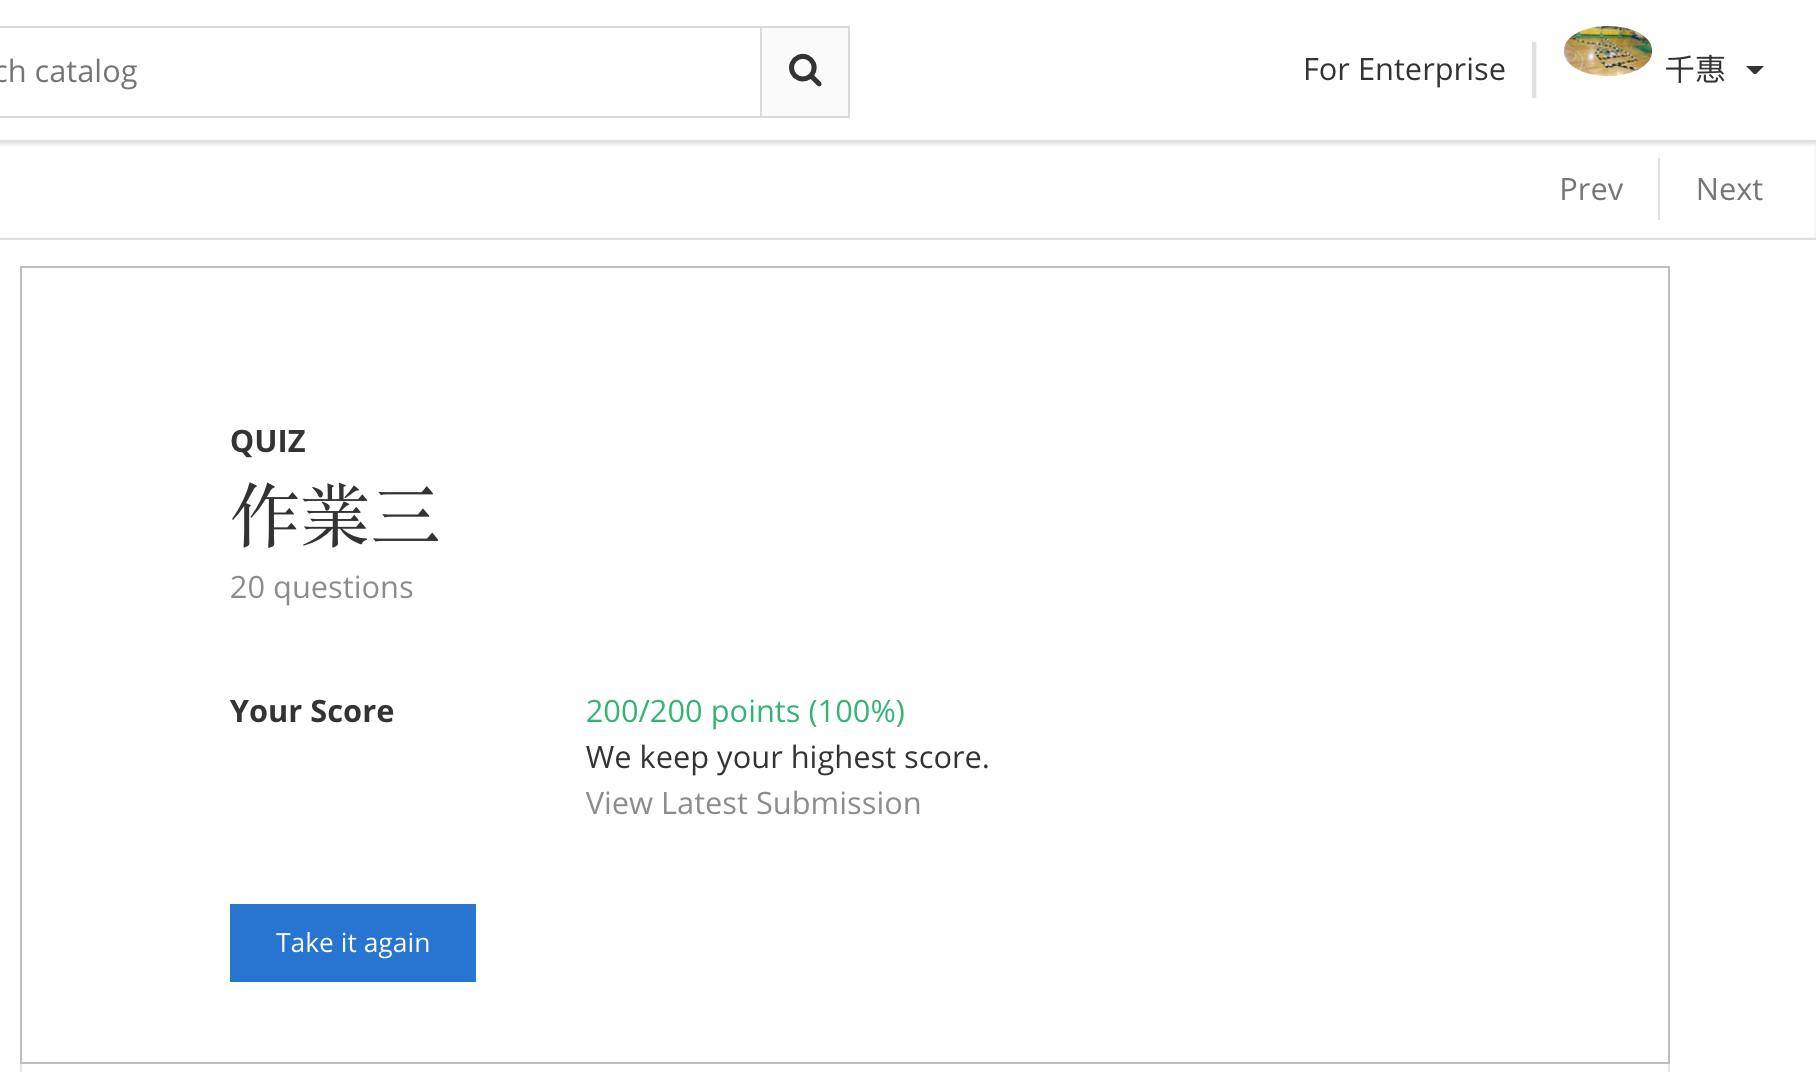
\includegraphics[width=16.5cm, keepaspectratio=true]{1.png}
	
	\section*{Problem 2}
		\vspace{-1em}
		\begin{flalign*} 
		H &= X(X^TX)^{-1}X^T\\
		H^2 &= X(X^TX)^{-1}X^TX(X^TX)^{-1}X^T \\ 
			&=X(X^TX)^{-1}(X^TX)(X^TX)^{-1}X^T 	&\text{(By commmutative law.)} \\
			&=X(X^TX)^{-1}X^T 					&(Since (X^TX)^{-1}(X^TX) = I)\\
			&=H 								&\text{(double projection = single one)}
		\end{flalign*}
		\vspace{-4em}
		\begin{flalign*} 
		(I-H)^2&=I^2-2IH+H^2=I-2H+H=I-H 		&\text{(double residual transform = single one)}
		\end{flalign*}

	\section*{Problem 3}
		Prove that SGD with $err({\bf w,x},y)=max(0, -y{\bf w}^T{\bf x})$ results in PLA.\\
		PLA: ${\bf w}_{t+1} \leftarrow {\bf w}_t+\llbracket y\neq sign({\bf w}_t^T{\bf x})\rrbracket(y{\bf x}) = {\bf w}_t+(err_{0/1})(y{\bf x})$\\
		SGD: ${\bf w}_{t+1} \leftarrow {\bf w}_t-\nabla err({\bf w, x}, y)$\\
		When $y=+1$ and ${\bf w}_t^T{\bf x} > 0,
		\begin{cases}
		err_{0/1} = 0 \Rightarrow {\bf w}_{t+1}\leftarrow {\bf w}_t\\
		err({\bf w,x},y)=0 \Rightarrow\nabla err({\bf w,x},y)=0 \Rightarrow {\bf w}_{t+1}\leftarrow {\bf w}_t \\
		\end{cases}$\\
		When $y=+1$ and ${\bf w}_t^T{\bf x} < 0,
		\begin{cases}
		err_{0/1} = 1 \Rightarrow {\bf w}_{t+1}\leftarrow {\bf w}_t+{\bf x}\\
		err({\bf w,x},y)= -{\bf w}^T{\bf x}\Rightarrow\nabla err({\bf w,x},y)=-{\bf x} \Rightarrow {\bf w}_{t+1}\leftarrow {\bf w}_t+{\bf x} \\
		\end{cases}$\\
		When $y=-1$ and ${\bf w}_t^T{\bf x} > 0,
		\begin{cases}
		err_{0/1} = 1 \Rightarrow {\bf w}_{t+1}\leftarrow {\bf w}_t-{\bf x}\\
		err({\bf w,x},y)= {\bf w}^T{\bf x}\Rightarrow\nabla err({\bf w,x},y)={\bf x} \Rightarrow {\bf w}_{t+1}\leftarrow {\bf w}_t-{\bf x} \\
		\end{cases}$\\
		When $y=-1$ and ${\bf w}_t^T{\bf x} < 0,
		\begin{cases}
		err_{0/1} = 0 \Rightarrow {\bf w}_{t+1}\leftarrow {\bf w}_t\\
		err({\bf w,x},y)=0 \Rightarrow\nabla err({\bf w,x},y)=0 \Rightarrow {\bf w}_{t+1}\leftarrow {\bf w}_t \\
		\end{cases}$\\
		$\Rightarrow$ SGD with $err({\bf w,x},y)=max(0, -y{\bf w}^T{\bf x})$ results in PLA.

	\section*{Problem 4}
		To minimize $\hat{E}_2(\Delta u,\Delta v)$, we would ideally like to find $\Delta u$ and $\Delta v$ such that $\nabla\hat{E}_2(\Delta u,\Delta v)=0$.\\
		This is the same as finding $\begin{bmatrix}\Delta u\\ \Delta v\end{bmatrix}$ such that $\nabla E(u+\Delta u, v+\Delta v)=\begin{bmatrix}0\\0\end{bmatrix}$.\\
		$E(u+\Delta u,v+\Delta v)\approx \hat{E}_2(\Delta u,\Delta v) = b_{uu}(\Delta u)^2+b_{vv}(\Delta v)^2+b_{uv}(\Delta u)(\Delta v)+b_u\Delta u+b_v\Delta v+b$
		\begin{flalign*}
		\Rightarrow \nabla E(u+\Delta u,v+\Delta v) &\approx\
		\begin{bmatrix}b_u+b_{uu}\Delta u+b_{uv}\Delta v\\b_v+b_{uv}\Delta u+b_{vv}\Delta v\end{bmatrix}
		= \begin{bmatrix}b_u\\b_v\end{bmatrix} +
		\begin{bmatrix}b_{uu} & b_{uv}\\b_{uv} & b_{vv}\end{bmatrix} * 
		\begin{bmatrix}\Delta u\\\Delta v\end{bmatrix}&\\
		&= \nabla E(u,v)+\nabla^2E(u,v) \begin{bmatrix}\Delta u\\\Delta v\end{bmatrix}&
		\end{flalign*}
		$0 = \nabla E(u+\Delta u,v+\Delta v) \approx \nabla E(u,v)+\nabla^2E(u,v)
		\begin{bmatrix}\Delta u\\\Delta v\end{bmatrix} \\
		\Rightarrow \begin{bmatrix}\Delta u\\\Delta v\end{bmatrix} = -(\nabla^2E(u,v))^{-1}\nabla E(u,v)$
	\vspace{-0.1em}
	\section*{Problem 5}
		likelihood(logistic h) $\propto \prod\limits_{n=1}^{N} h_y({\bf x}_n) 
		\propto \ln \prod\limits_{n=1}^{N} h_y({\bf x}_n)$
		\begin{flalign*}
			\text{max likelihood(logistic h)}
			&\rightarrow \max\limits_{h}\hspace{0.5em}\ln \prod\limits_{n=1}^{N} h_y({\bf x}_n) &\\
			&\rightarrow -\min\limits_{h}\hspace{0.5em}\dfrac{1}{N}\ln \prod\limits_{n=1}^{N} h_y({\bf x}_n) &\\
			&\rightarrow -\min\hspace{0.5em}\dfrac{1}{N}\ln \prod\limits_{n=1}^{N} \dfrac{e^{{\bf w}_{y_n}^T {\bf x}_n}}{\sum\limits_{i=1}^K e^{{\bf w}_i^T {\bf x}_n}} &\\
			&\rightarrow -\min\hspace{0.5em}\dfrac{1}{N}\ln \prod\limits_{n=1}^{N} e^{{\bf w}_{y_n}^T {\bf x}_n} - \ln \prod\limits_{n=1}^{N}(\sum\limits_{i=1}^K e^{{\bf w}_i^T {\bf x}_n}) &\\
			&\rightarrow -\min\hspace{0.5em}\dfrac{1}{N}\sum\limits_{n=1}^{N} {\bf w}_{y_n}^T {\bf x}_n - \sum\limits_{n=1}^{N}\ln (\sum\limits_{i=1}^K e^{{\bf w}_i^T {\bf x}_n}) &\\
			&\rightarrow \min\hspace{0.5em}\dfrac{1}{N}\sum\limits_{n=1}^{N}\Big(\ln(\sum\limits_{i=1}^K e^{{\bf w}_i^T {\bf x}_n})-{\bf w}_{y_n}^T {\bf x}_n \Big)
		\end{flalign*}
		$E_{in}({\bf w}_1,{\bf w}_2,...{\bf w}_K) = \dfrac{1}{N}\sum\limits_{n=1}^{N}\Big(\ln(\sum\limits_{i=1}^K e^{w_i^T {\bf x}_n})-{\bf w}_{y_n}^T {\bf x}_n \Big)$

	\vspace{-0.3em}
	\section*{Problem 6}
		\begin{flalign*}
			\dfrac{\partial E_{in}}{\partial{\bf w}_i} &= \dfrac{\partial\Big[\dfrac{1}{N}\sum\limits_{n=1}^{N}\Big(\ln (\sum\limits_{i=1}^K e^{{\bf w}_i^T {\bf x}_n})-{\bf w}_{y_n}^T {\bf x}_n \Big)\Big]}{\partial{\bf w}_i} &\\
			&= \dfrac{1}{N}\sum\limits_{n=1}^{N}\Big[\Big(\dfrac{1}{\sum\limits_{i=1}^K e^{{\bf w}_i^T {\bf x}_n}}\cdot e^{{\bf w}_i^T {\bf x}_n}\cdot {\bf x}_n\Big)- \llbracket y_n=i \rrbracket\cdot{\bf x}_n\Big] \\
			&= \dfrac{1}{N}\sum\limits_{n=1}^{N}\Big((h_i({\bf x}_n)- \llbracket y_n=i \rrbracket)\cdot {\bf x}_n \Big)
			&\Big(\text{Since } \dfrac{1}{\sum\limits_{i=1}^K e^{{\bf w}_i^T {\bf x}_n}}\cdot e^{{\bf w}_i^T{\bf x}_n} = h_i({\bf x}_n)\Big)
		\end{flalign*}
	
	\section*{Problem 7}
		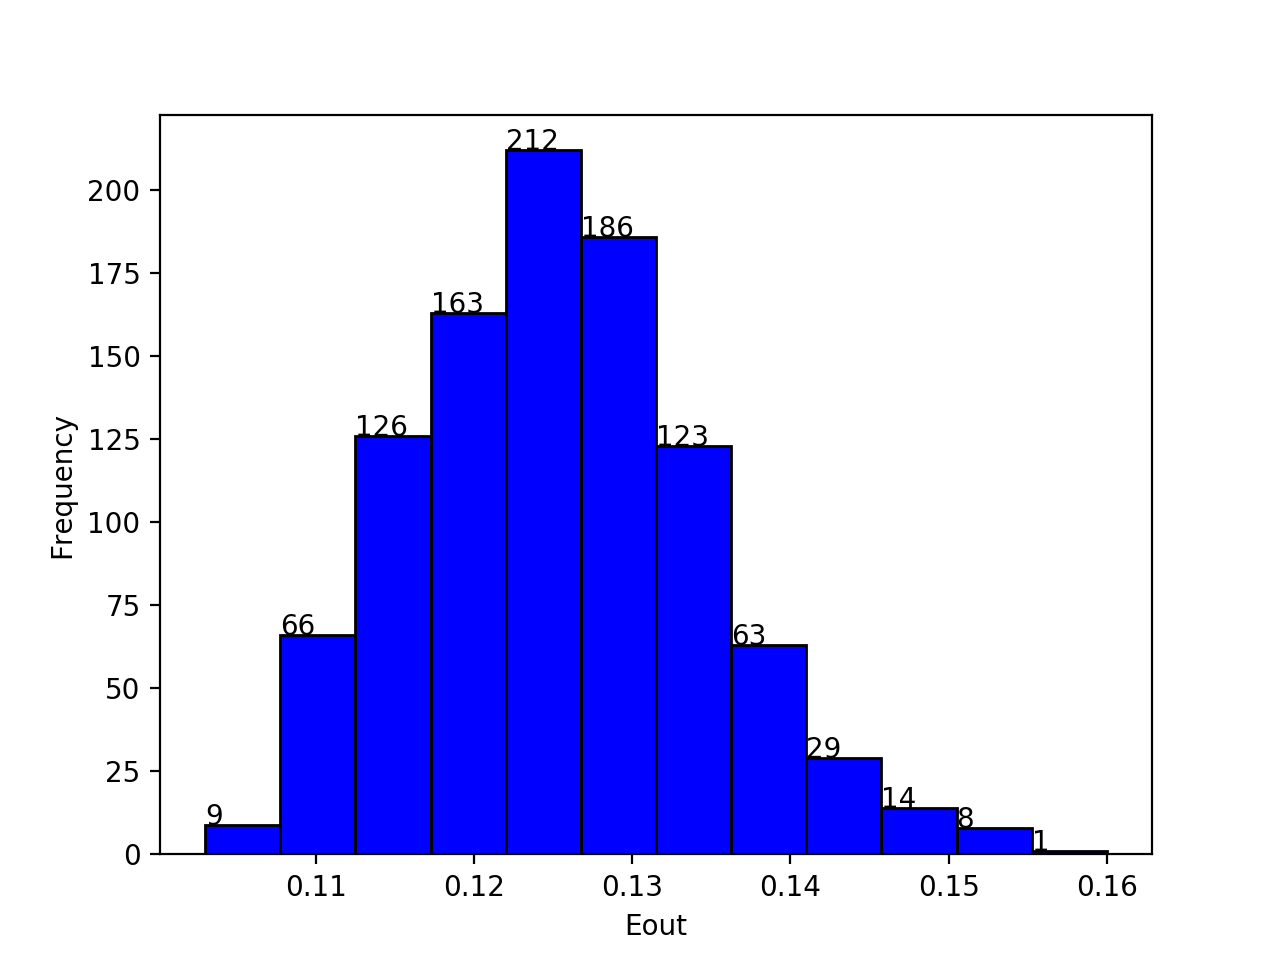
\includegraphics[width=17cm, keepaspectratio=true]{7.png}

	\newpage
	\section*{Problem 8}
		$GD-Ein: 0.467 \rightarrow 0.464 \\
		SGD-Ein: 0.467 \rightarrow 0.198 $\\
		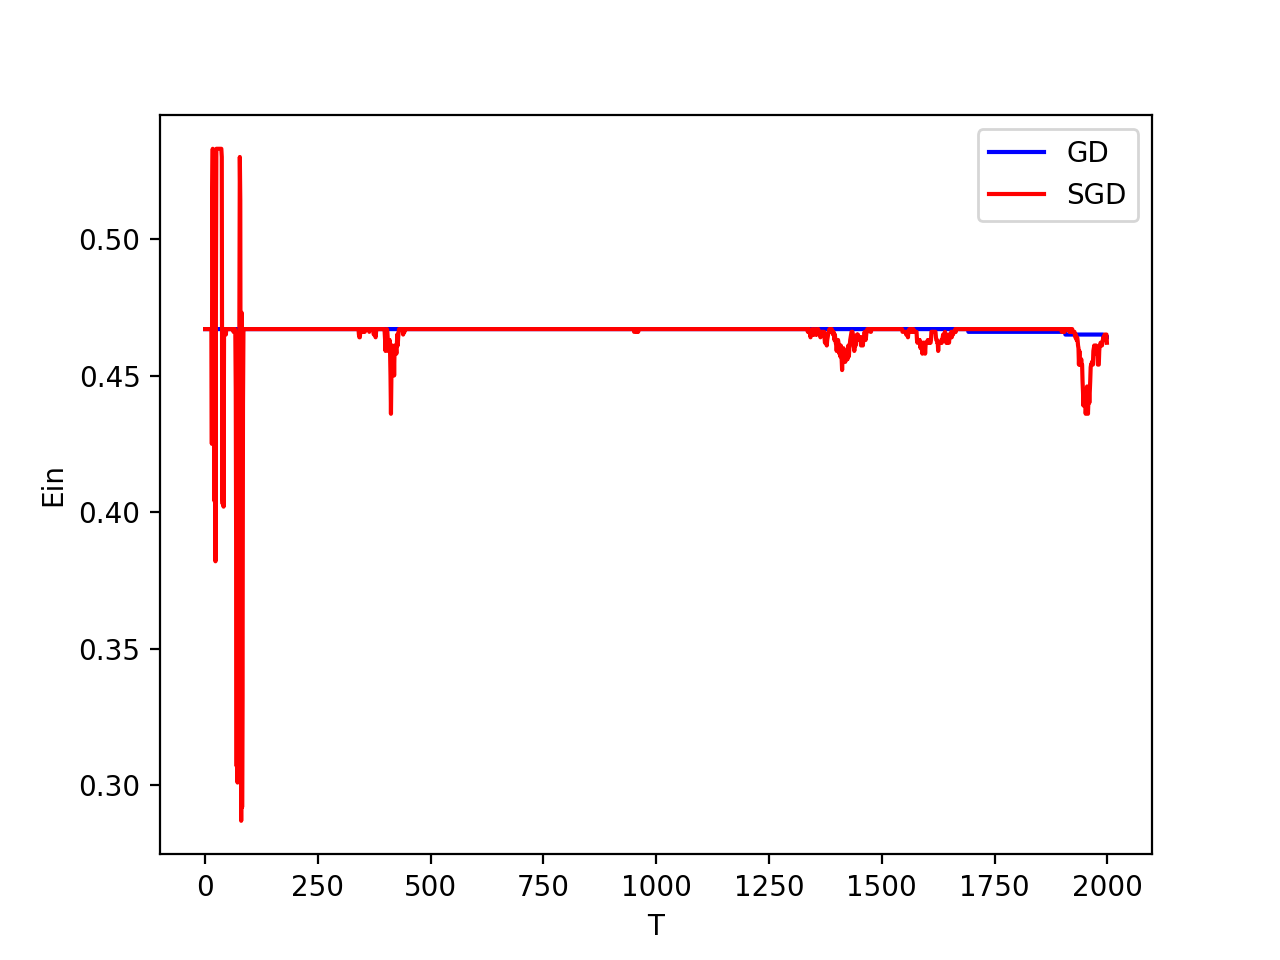
\includegraphics[width=14cm, keepaspectratio=true]{ein_8.png}\\
		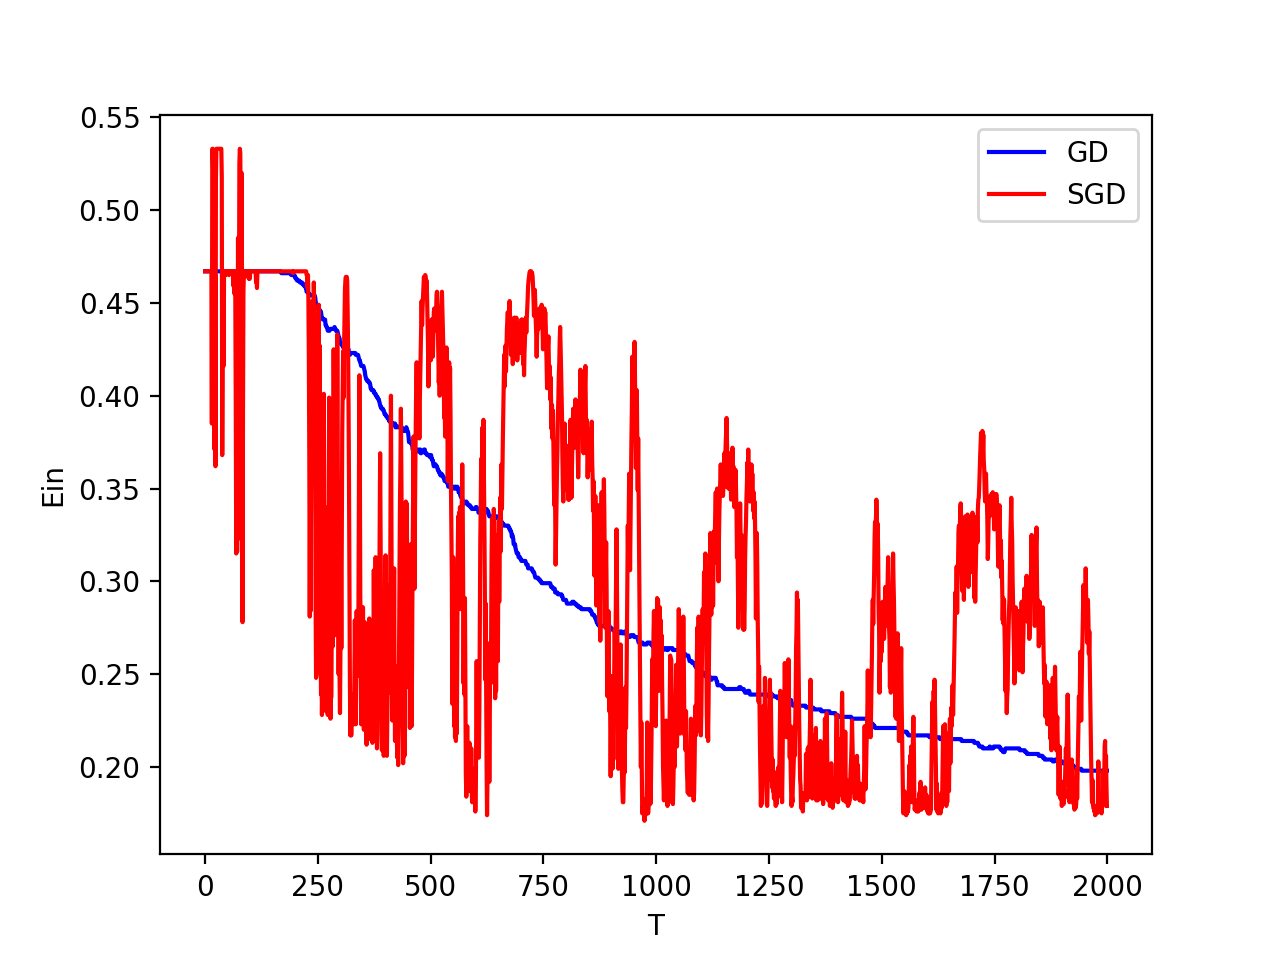
\includegraphics[width=14cm, keepaspectratio=true]{ein_9.png}
	
	\section*{Problem 9}
		$GD-Eout: 0.477 \rightarrow 0.4716\\
		SGD-Eout: 0.477 \rightarrow 0.2206$ \\
		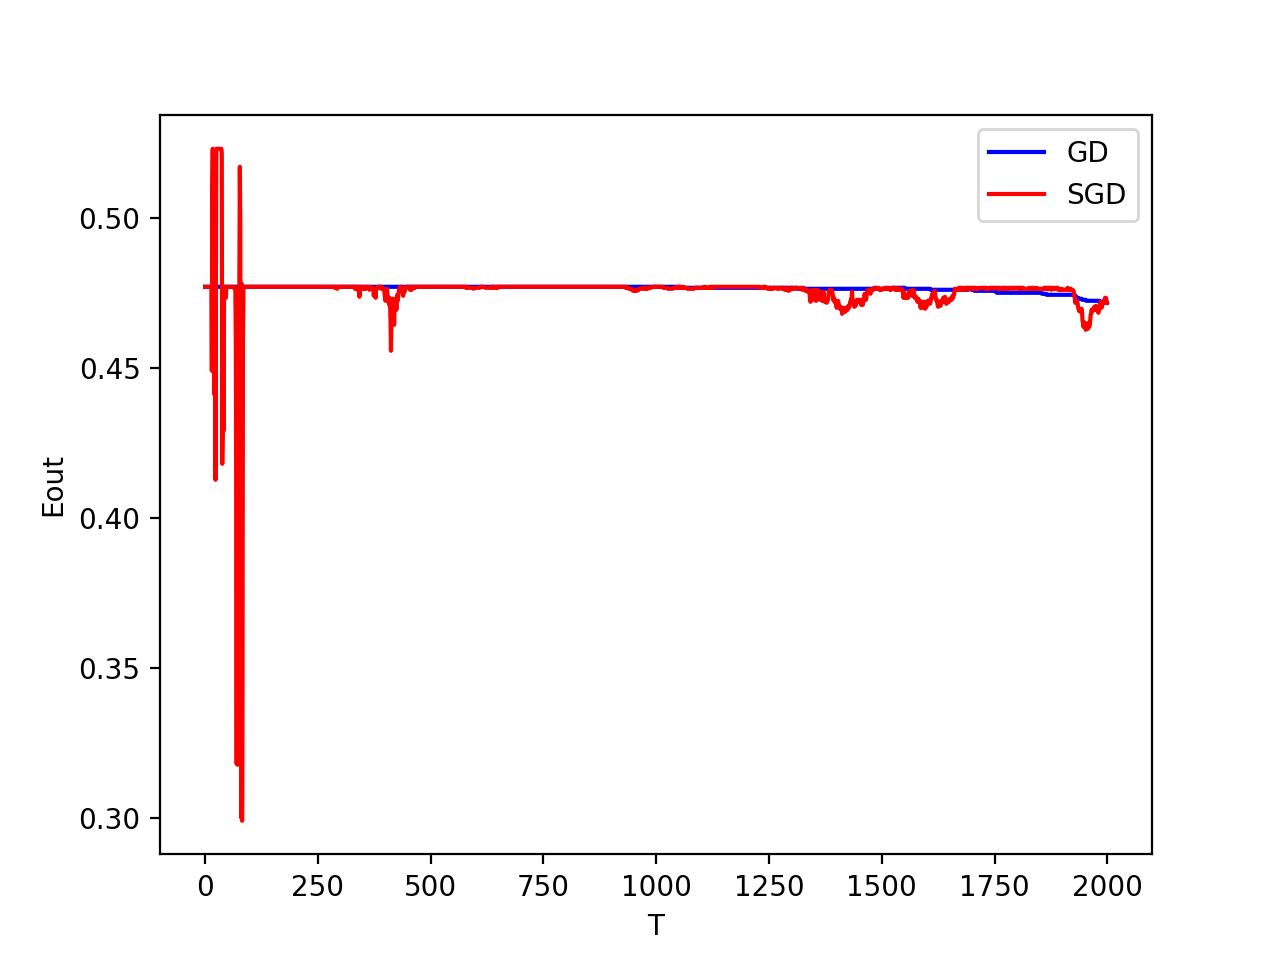
\includegraphics[width=14cm, keepaspectratio=true]{eout_8.png}\\
		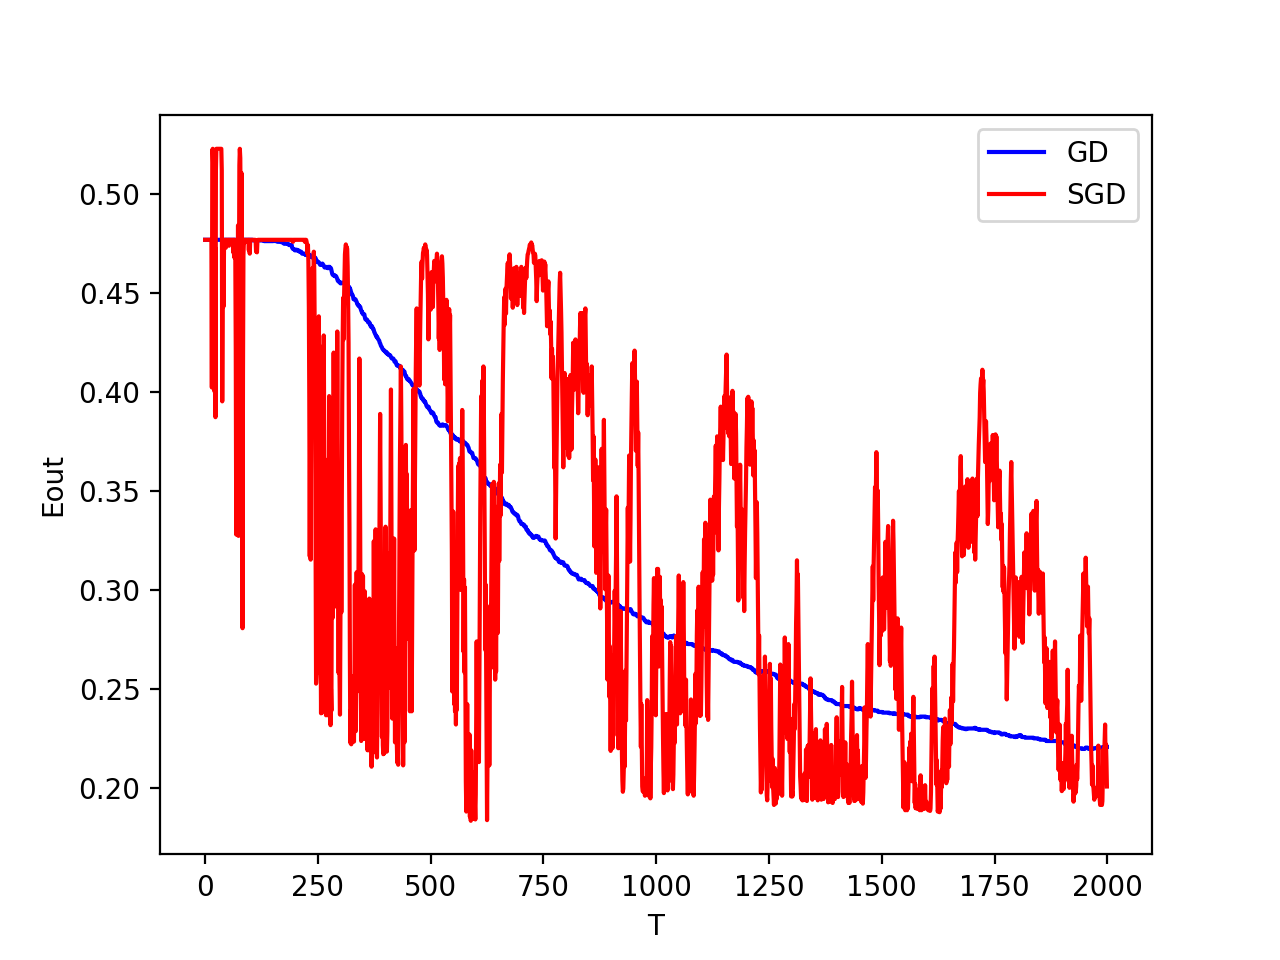
\includegraphics[width=14cm, keepaspectratio=true]{eout_9.png}


	\section*{Problem 10(Bonus)}
	\subsection{}
		\begin{flalign*} 
		% X = U\Gamma V^T \\
		% U^TU = I\rho \\
		% V^TV = I\rho \\
		% {\bf w}_{lin} = V\Gamma^{-1}U^T {\bf y} \\
		X^TX{\bf w}_{lin}
			&= X^T(U\Gamma V^T)(V\Gamma^{-1}U^T {\bf y}) \\ 
			&= X^TU\Gamma (V^TV)\Gamma^{-1}U^T {\bf y} 	&\text{(By commmutative law.)} \\
			&= X^TU(\Gamma\Gamma^{-1})U^T {\bf y} 	&\text{(Since }V^TV = I\rho)\\
			&= X^T(UU^T) {\bf y}					&\text{(Since }\Gamma\Gamma^{-1} = I\rho)\\
			&= X^T{\bf y} 							&\text{(Since }U^TU = I\rho)
		\end{flalign*}
		
	% \subsection{}
	% 	Given $Xw=y$, we have to proof that $w = X^+y = V\Gamma U^Ty$ has the smallest norm.
	% 	\begin{flalign*}
	% 		\norm{Xw-y}	&= \norm{U\Gamma V^Tw-y} &\text{(Since }X=U\Gamma V^Tw) &\\
	% 						&= \norm{\Gamma V^Tw-U^Ty} &\text{(Since V is isometry and }V^{-1}=V^T)
	% 	\end{flalign*}
	% 	\begin{flalign*}
	% 		&\text{Let } z = V^Tw 
	% 		\Rightarrow \norm{z}= \norm{w} &\text{(Since V is isometry.)}&\\
	% 		&\norm{Xw-y} = \norm{\Gamma z-U^Ty}&\\
	% 		&\Rightarrow z = \Gamma^{-1}U^Ty \text{ minimize } \norm{z-\Gamma^{-1}U^Ty} \text{ and thus minimize } \norm{Xw-y} &\\
	% 		&z=V^Tw=\Gamma^{-1}V^Ty \Rightarrow w = V\Gamma^{-1}U^Ty = X^+y &\\
	% 		&\Rightarrow w = X^+y = w_{lin} \text{ minimize } \norm{Xw-y} &\\
	% 		&\Rightarrow w_{lin} \text{ is the shortest weight vector that minimizes } E_{in} 
	% 	\end{flalign*}

		

	\clearpage
	\end{CJK}
\end{document}